% Created 2021-12-27 Mon 23:06
% Intended LaTeX compiler: pdflatex
\documentclass[11pt]{article}
\usepackage[utf8]{inputenc}
\usepackage[T1]{fontenc}
\usepackage{graphicx}
\usepackage{grffile}
\usepackage{longtable}
\usepackage{wrapfig}
\usepackage{rotating}
\usepackage[normalem]{ulem}
\usepackage{amsmath}
\usepackage{textcomp}
\usepackage{amssymb}
\usepackage{capt-of}
\usepackage{hyperref}
\usepackage[margin=.5in]{geometry}
\author{Sreejith Sreekumar}
\date{\today}
\title{Stat Definitions}
\hypersetup{
 pdfauthor={Sreejith Sreekumar},
 pdftitle={Stat Definitions},
 pdfkeywords={},
 pdfsubject={},
 pdfcreator={Emacs 27.2 (Org mode 9.4.4)}, 
 pdflang={English}}
\begin{document}

\maketitle
\tableofcontents




\section{\underline{Confidence Interval}}
\label{sec:org8fbec10}
\begin{itemize}
\item A confidence interval gives the PROBABILITY that our true value lies within the range of values. Bigger interval = higher probability
\end{itemize}

\section{\underline{Probability}}
\label{sec:org74be2e8}
\begin{itemize}
\item Area under an interval of a distribution curve.
\end{itemize}

\section{\underline{Likelihood} vs Probability}
\label{sec:org94b6264}

\begin{itemize}
\item \href{https://stats.stackexchange.com/a/183885/84189}{Answer from Cross Validated}
Likelihood: What is the best values of the parameters so that the data that we observed follows a <some> distribution?
Probability: Assuming that the data comes from a certain distribution what is the chance. Probability is the area under the PDF curve
\end{itemize}

\section{\underline{Percentage of normal distribution lies within 1 std of mean? 2, 3 std?}}
\label{sec:orgff1049d}
\begin{itemize}
\item 68\%, 95\%, 99.7\%
\end{itemize}

\section{\underline{SGD Update Rule}}
\label{sec:orgc7e8bb9}

$$\theta = \theta - \alpha \Delta J(\theta)$$
$$(Current\ \theta \ vector) - learning\ rate * (Gradient\ of\ Slope)$$

\section{\underline{Probability and Statistics}}
\label{sec:org937ff47}

The problems considered by probability and statistics are inverse to each other.
In probability theory we consider some underlying process which has some randomness or uncertainty modeled by random variables, and we figure out what happens.
In statistics we observe something that has happened, and try to figure out what underlying process would explain those observations.

\section{\underline{Law of Large Numbers}}
\label{sec:org6637a8b}

If you repeat an experiment independently a large number of times and average the result, what you obtain should be close to the expected value

\section{\underline{Central Limit Theorem}}
\label{sec:orgd3aa75e}

\section{\underline{Type I and Type II Error}}
\label{sec:org31774ea}

Type 1: False Positive, Type 2: False Negative

\section{\underline{Inverse Document Frequency}}
\label{sec:orgc9672ea}

$$idf = log \frac{|D|}{d : ti \in d}$$
where | D | is the number of documents in our corpus, and | \{d : ti \(\in\) d\} | is the number of documents in which the term appears.

\section{\underline{Kolmogorov - Smirnov Test}}
\label{sec:org9316ccb}

Tests whether sample fits a distribution well.

\section{\underline{Normal Distribution Standard Deviations}}
\label{sec:org79bb30d}

\begin{center}
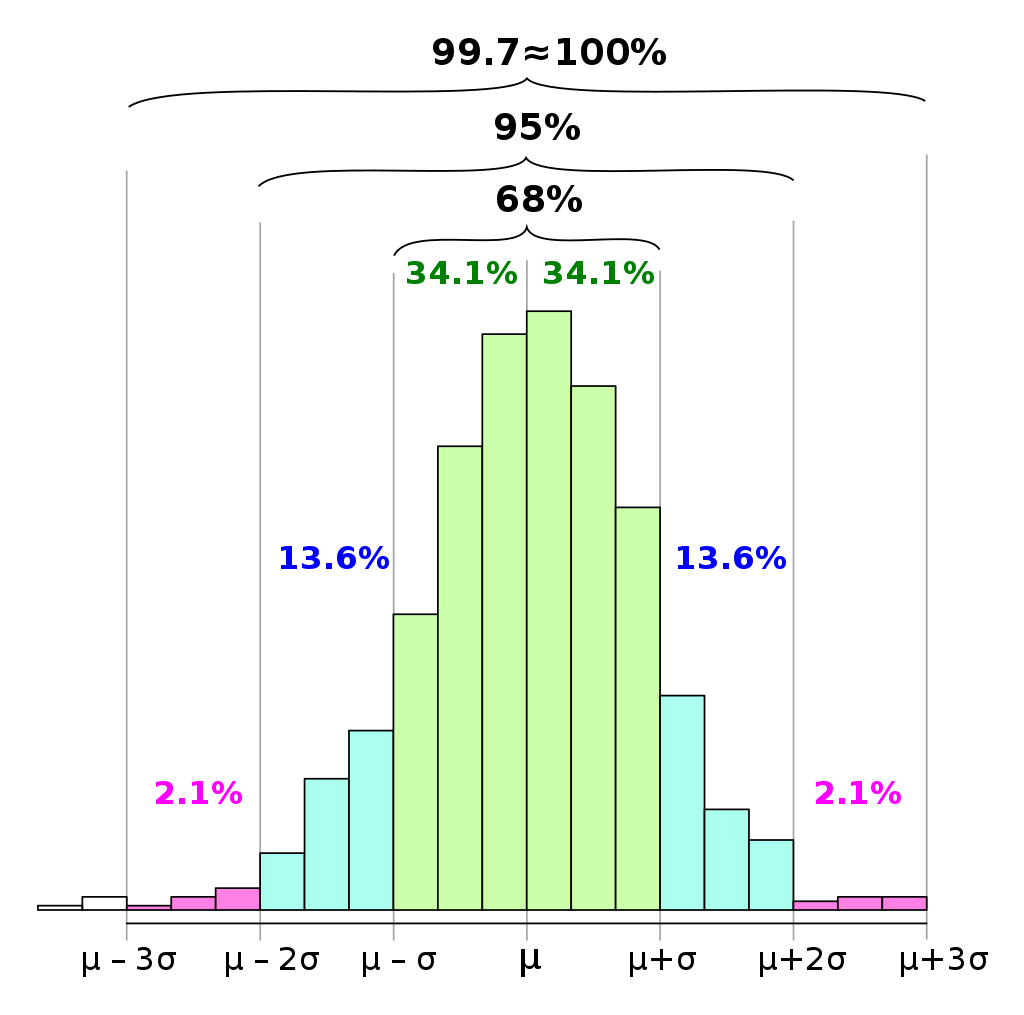
\includegraphics[width=.9\linewidth]{normal-sd.png}
\end{center}

\section{\underline{Confidence Interval}}
\label{sec:orgca8dcda}

There are 100 products and 25 of them are bad. What is the confidence interval? \\

p = 25/100 = 0.25 \\

CI = 0.25 +/- 1.96 sqrt( (0.25(1-0.25)) * 100) \\

CI = p +/- Z * sqrt(variance of binom dist) \\

CI = (16.5,33.5) \\

95\% confidence = plus or minus 1.96 STDEV

\subsection{\underline{Margin of Error}}
\label{sec:org5f06ddd}

Margin of Error = \(t * \frac{s}{\sqrt{n}}\)

\section{\underline{Isolation Forest}}
\label{sec:orgef19899}

Creates splits like a random forest, but find out how difficult is it to isolate the path to split an instance.
Answer: \href{https://www.quora.com/What-is-the-difference-between-random-forest-and-isolation-forest}{Quora}

\section{\underline{T-Test (Two Sample)}}
\label{sec:org51a5bcd}

\begin{itemize}
\item Both has to be normal distributions
\item Both needs to have similar variance
\item \(\sigma\) is unknown
\item Smaller sample sizes (Ideally in the range of 20-30) or else we use \textbf{\textbf{z-test}}
\item \(\frac{\bar{x1} - \bar{x2}}{\sqrt{\frac{s1^{2}}{n1} - \frac{s2^{2}}{n2}}}\)
\end{itemize}

\section{\underline{T-Test and Z-Test for one sample}}
\label{sec:orgd174654}

\begin{itemize}
\item T-test is used when the sample size is less than 30
\item t-Test = \(\frac{\bar{x} - \mu}{\frac{s}{\sqrt{n}}}\)
\item From CLT, as n increased sample sd will be similar to population sd \\
z-test = \(\frac{\bar{x} - \mu}{\frac{\sigma}{\sqrt{n}}}\)
\item when sample size is > 30 and \(\sigma\) is available, use \textbf{Z-test}, else use \textbf{T-Test}
\end{itemize}
\section{\underline{Chi-Squred Test}}
\label{sec:org5b7c362}

If there is a statistically significant difference in the observed vs expected counts.

\(\chi{2} = \Sigma\frac{(O_{i} - E_{i})^2}{E_{i}}\) \\


Example:

\noindent\rule{\textwidth}{0.5pt}
Coin tossed 50 times.

Expected: 25H 25T

Observed: 28H 22T \\


\(\frac{(28-25)^2}{25} +   \frac{(22-25)^2}{25}\) \\

\(= \frac{9}{25} + \frac{9}{25}\) \\

\(= \frac{18}{25}\) \\

\(= 0.72\) \\

H0: There is no statistically significant difference between observed values and expected values.

For a critical value of 0.05, and degree of freedom (n-1 = 1)   \(\chi^{2}\) = 3.84
Since this value is greater than 0.72, we accept Null Hypothesis


\section{\underline{Probability Distributions}}
\label{sec:org58448ba}

Mathematical Function that gives the probabilities of occurrence of different
possible outcomes for an experiment. \\

\subsection{Binomial:}
\label{sec:org22cfa61}

Coin toss event repeated n times, with probability p of success. 

\begin{itemize}
\item \(nCr . P^{r} . (1 - P)^{n-r}\)
\item Discrete with parameters (n, p)
\item n independent experiments
\item Success p
\item Failure (1-p)
\item Mean: np,
\item Median: \(\lfloor np \rfloor\), \(\lceil np \rceil\)
\end{itemize}

\subsection{Exponential}
\label{sec:org6fd6f0c}

\begin{itemize}
\item Exponential distribution is often concerned with the amount of time until some specific event occurs.
\item \(f(x) = me^{-mx}\)
\item Decay parameter, \(m = \frac{1}{\mu}\)
\item \(\mu = \sigma\)
\end{itemize}

\begin{verbatim}
import matplotlib.pyplot as plt
import numpy as np

def get_ex(m, x):
    return round(m * np.power(np.e, -m*x), 2)

points = [(x, get_ex(0.25, x)) for x in list(range(20))]

xs = [x[0] for x in points]
ys = [y[1] for y in points]

f, ax = plt.subplots()
ax.scatter(xs, ys)
ax.set_ylabel("f(x)")
ax.set_xlabel("mu = 4")
plt.show()
\end{verbatim}

\begin{center}
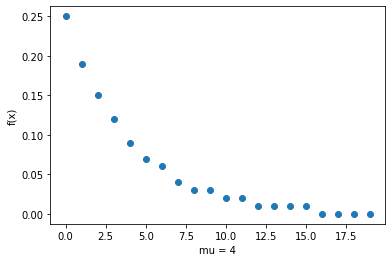
\includegraphics[width=10cm]{./obipy-resources/ZODX3e.png}
\end{center}

\section{\underline{Maximum Likelihood Estimation}}
\label{sec:orgcf5dcd8}

Location which maximizes the likelihood of the data we measured.


Likelihood given all data points

L(\(\mu\), \(\sigma\)| x1, x2,\ldots{},xn) =  L(\(\mu\), \(\sigma\)| x1) *  L(\(\mu\), \(\sigma\)| x2)\ldots{}

\begin{itemize}
\item Take derivative wrt \(\mu\) , and treat \(\sigma\) like it is constant; and equate it to 0
\item Take derivate wrt \(\sigma\), and treat \(\mu\) like it is a constant
\item Take ln
\item MLE calculation of Normal Distribution:

\href{./mle-normal-dist.pdf}{Derivation}
\end{itemize}

\section{\underline{EM Algorithms}}
\label{sec:org60e8452}

Goal: \(\theta_{MLE} \in argmax_{\theta}P_{\theta}(x)\)
Problem: \(P_{\theta}(x) = \sum_{x} P_{\theta}(x)\) is difficult to maximize

\begin{itemize}
\item Start with a random estimate (and random parameters)
\item Observe the data
\item Adjust the parameters to some data so that the estimates of the parameter are better
\item Observe more data
\item Adjust \ldots{}
\end{itemize}

\section{\underline{Multicollinearity}}
\label{sec:org898ce17}

\begin{itemize}
\item Measured by VIF
\item Regress one variable with other variables: \(\frac{1}{1-R^{2}}\)
\item VIFs are calculated by taking a predictor, and regressing it against every other predictor in the model.
\item Useful Link: \url{https://etav.github.io/python/vif\_factor\_python.html}
\item 

\item Any variable with VIF > 5 must be removed
\end{itemize}
\end{document}
